\documentclass[11pt]{article}
\usepackage[T1]{fontenc}
\usepackage[utf8]{inputenc}
\usepackage[english]{babel}

\usepackage{graphicx}
\graphicspath{ {./img/} }

\begin{document}

\section{Results}


For the very first tries we tried to make a large, VGG-16 like network. With 16 convolution layers, from 32 filters to 512, and two Dense layers. We managed to reach incredible validation accuracy.
\\\
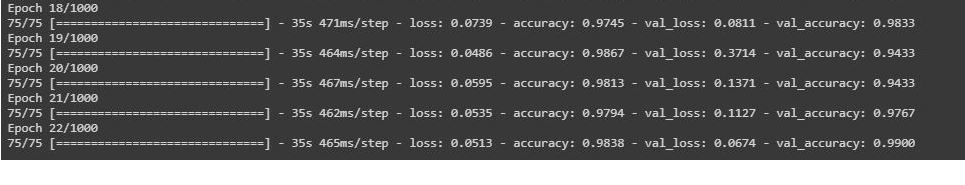
\includegraphics[scale=0.5]{over_fit_1}
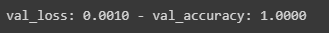
\includegraphics[scale=0.5]{limitless_overfitting}
\\\
After evaluation, it turned out that it was probably just overfitting, as the model performed terrible. I am unsure why the validation accuracy kept increasing too, perhaps the validation data was picked unluckily and was too easy to categorise compared to the training data. (I could even imagine that some of the pictures somehow ended up in both folders)

Later we tried a smaller and smaller conv net. I tried a net with 10 layers, double convolution layers before each pooling. This was probably still learning too quickly and start overfitting.
\\\
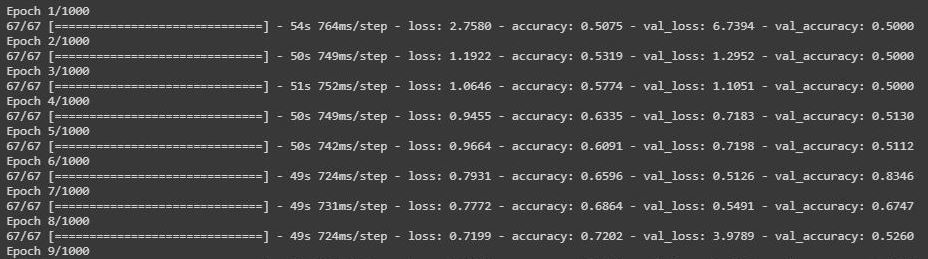
\includegraphics[scale=0.5]{double}
\\\

In the end we ended up with a simple model with single conv layers (filters form 64 to 1024), which performed reasonably well.

The final model's second round of training(there was no validation):
\\\
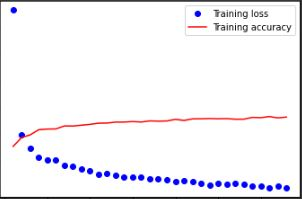
\includegraphics[scale=0.5]{long_train}
\\\
And the final evaluation:
\\\
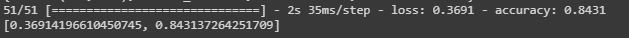
\includegraphics[scale=0.5]{eval}

\end{document}